\documentclass[12pt,fleqn]{article}\usepackage{../../common}
\begin{document}
Ders 8

Bu derste lineer denklemleri tamamen çözmeyi öğreneceğiz, amaç, eğer bir
çözüm var ise $Ax=b$ çözümü olacak. Bir çözümün olmaması da mümkündür,
eliminasyon kullanarak bu olasılığı saptamayı da öğreneceğiz. Eğer çözüm
var ise, bu çözüm tek çözüm müdür, bir çözüm ailesi var mıdır? Bunlara
bakacağız. 

Örnek olarak önceki derste sıfır uzayı bulmak için kullandığım örneği
kullanacağım, sadece sağ tarafta sıfır yerine $b$ vektörü var.

$$ x_1 + 2x_2 + 2x_3 + 2x_4 = b_1 $$

$$ 2x_1 + 4x_2 + 6x_3 + 8x_4 = b_2 $$

$$ 3x_1 + 6x_2 + 8x_3 + 10x_4 = b_3 $$

Hatırlarsak bu örnekte 3. satır 1. ve 2. satırın toplamıydı. Bu bilgiden
hareketle eliminasyon bu denklem sisteminin sağ kısmı hakkında bir şey
keşfedeceğini hemen tahmin edebiliriz. Mesela $b_1=1,b_2=5,b_3=17$ desem,
bu deklemin çözümü olmaz. Çoğu sayı için aslında bu denklemin çözümü
olmaz. Hangi $b$'ler için çözüm olabilir? Mesela $b_1=1,b_2=5,b_3=6$
deseydim çözüm olurdu, çünkü o zaman denklemin sağ tarafında da 1. ve
2. satır toplamı 3. satıra eşit olurdu, aynen sol tarafta olduğu
gibi. Eliminasyonun bu durumu nasıl keşfedeceğini görelim bakalım.

Denklem sistemini matris formunda yazalım, eşitliğin sağ kısmını da
matrisin sağına bitiştirelim, ki bu eklemlenmiş (augmented) bir matris
olacak, 

$$ 
\left[\begin{array}{rrrr|r}
1 & 2 & 2 & 2 & b_1 \\
2 & 4 & 6 & 8 & b_2 \\
3 & 6 & 8 & 10 & b_3
\end{array}\right]
 $$

Bunu eliminasyon sırasında aynı işlemleri eşitliğin sağ kısmına da rahatça
uygulayabilmek için yaptık. Eliminasyona başlayalım; Pivot en üst sol
kısımda, 1. satırdan 2 taneyi 2., 3 taneyi 3. satırdan çıkartırım,

$$ 
\left[\begin{array}{llll|l}
(1) & 2 & 2 & 2 & b_1 \\
0 & 0 & 2 & 4 & b_2-2b_1 \\
0 & 0 & 2 & 4 & b_3-3b_1
\end{array}\right]
 $$

Bir sonraki pivot'a geçiyorum, ve 2. satırı 3.'den çıkartıyorum,

$$ 
\left[\begin{array}{llll|l}
(1) & 2 & 2 & 2 & b_1 \\
0 & 0 & (2) & 4 & b_2-2b_1 \\
0 & 0 & 0 & 0 & b_3-b_2-b_1
\end{array}\right]
 $$

En son satırdaki formül ne diyor? 

$$ 0 = b_3 - b_2 - b_1 $$

Bu formül bu sistemin ``çözülebilme (solvability)'' koşulunu da tarif
ediyor. Bu durumu zaten üstte tahmin etmiştik, şimdi eliminasyon da
keşfetti. Üstteki ifade son denklem hakkında bir beyanda bulundu. Şimdi
geri kalan (ilk) iki denklemi dört bilinmeyen üzerinden çözmeye
uğraşacağım.

Çözülebilme (eşitliğin sağ tarafı hakkında bir kural)

Eğer $b$ $C(A)$ içinde, yani $A$'nin kolon uzayında ise çözülebilir
demektir. 

Aynı şeyi farklı bir dille belirtelim;

$A$'nin hangi satır kombinasyonu sıfır sonucu veriyorsa, aynı kombinasyon,
$b$ üzerinde de sıfır sonucunu vermelidir. 

Tabii daha genel bir soru şu: bu sistemin çözümü var mıdır? Varsa, bu
çözümü nasıl buluruz? 

Tüm çözümleri bulmadan önce, tek bir çözümü bulmaya odaklanalım. Elimde iki
denklem var, 4 bilinmeyen var, aslında bir sürü çözüm bulmayı beklerim, ama
ondan önce, dediğimiz gibi, tek bir çözüm bulalım. Bu çözüme $x_{ozel}$
diyelim (particular, özel anlamında). 

1) Tüm serbest değişkenlere sıfır ver. 

2) $Ax=b$'nin pivot değişkenlerini çöz

Bu sistemde serbest değişkenler hangileri? Üstte eliminasyon sırasında bu
ortaya çıktı zaten, yeşille işaretli olanlar pivot, geri kalanları
serbest. Serbest değişkenler $x_2,x_4$. Bunlara sıfır verelim,
$x_2=0,x_4=0$, ayrıca $b_1=1,b_2=3,b_3=0$ olarak alalım,

$$ x_1 + 2x_3 = 1 $$

$$ 2x_3 = 3 $$

Geriye koyma tekniği ile $x_3 = 3/2$ ve bunu alıp iki üstteki denkleme
verince, $x_1 = -2$. Yani,

$$ x_{ozel} = \left[\begin{array}{c}
-2 \\ 0 \\ 3/2 \\ 0
\end{array}\right] $$

Bu özel çözüm, ``serbest değişkenlerinde sıfır olan özel çözüm'' daha doğrusu. 

Geri kalan çözümleri nasıl bulurum?  Şöyle, 

$$ x = x_{ozel} + x_{sıfır} $$

Yani $A$'nin sıfır uzayından herhangi bir vektör $x_{sıfır}$'i $x_{ozel}$
çözüme eklersem, tüm çözümleri teker teker bulmuş olurum. 

Bu niye işliyor? Ve bu kalıbın tekrar tekrar matematiğin geri kalanında
ortaya çıktığını göreceksiniz; sebep nedir? Düşünürsek, $Ax_{ozel} = b$
değil mi? Çünkü özel çözüm eşitliğin sağ tarafını tatmin eden
çözümdür. Diğer yandan $Ax_{sıfır} = 0$. Bunları toplarsam,

$$ Ax_{ozel} = b $$
$$ Ax_{sıfır} = 0 $$
$$ \underline{+\hspace{10em}} $$
$$ A(x_{ozel} + x_{sıfır}) = b $$

Sözel olarak belirtmek gerekirse, elimde bir çözüm var ise, öne sıfır
uzayından herhangi bir vektörü eklersem yeni bir çözüm elde ederim, çünkü
bu ekleme işlemi eşitliğin sağ tarafını değiştirmez / bozmaz, $b$'ye sıfır
ekleyince yine $b$ elde ederim. Üstteki örnek için bunu uyguluyalım, 

$$ 
x_{tum} = 
\left[\begin{array}{r}
-2 \\ 0 \\ \frac{3}{2} \\ 0
\end{array}\right] + 
c_1 
\left[\begin{array}{r}
-2 \\ 1 \\ 0 \\ 0
\end{array}\right] + 
c_2 
\left[\begin{array}{r}
2 \\ 0 \\ -2 \\ 1
\end{array}\right] 
 $$

$c_1,c_2$'nin çarptığı vektörleri daha önceki derste (aynı) $A$'nin sıfır
uzayında olarak bulmuştuk, onları direk alıp kullandık. Ayrıca onların tüm
kombinasyonlarını kullandık çünkü $x_{sıfır}$'in, yani sıfır uzayının tanımı
budur.

Soru: üstteki formülde ilk terimi oluşturan matrisi, yani $x_{ozel}$
kısmını bir sabit ile çarpmam gerekir mi? Cevap hayır, çünkü bu özel çözüm
bana $b$ sonucunu verdi, onu değiştirmem mümkün değil. Fakat $x_{sıfır}$'i
istediğim sabitle çarparım çünkü o eşitliğin sağ tarafı sıfır, sıfırla
sabit çarpılınca yine sıfır elde edilir. Tekrarlamak gerekirse, $x_{ozel}$
tek, ``özel'' bir vektör, $x_{sıfır}$ ise tüm bir .. altuzay (subspace)
değil mi? Yani tek bir şey artı tüm bir altuzaydan bahsediyoruz.

Çizmeye uğrasayım, boyut dört, o zaman $\mathbb{R}^4$'deyiz. Peki çözümümüz
bir altuzay oluşturur mu? Hayır. Özel çözüme eklediğimiz sıfır uzayı bir
altuzaydır, elimizde iki vektör var, yani $\mathbb{R}^4$'in içinde iki
boyutlu bir altuzaydayız bu durumda [hoca altta 4 boyutlu eksenler çizmeye
uğraştı, düzlem tüm çözümü gösteriyor, orijinden düzleme bir vektör çizdi
ki bu çözümlerden bir tanesi oluyor]

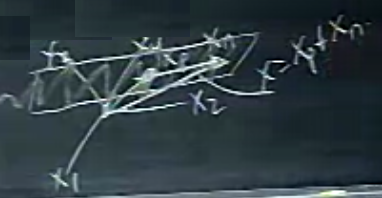
\includegraphics[height=5cm]{8_01.png}

Bu düzlem bir altuzay değil, dikkat, çünkü orijinden geçmiyor. 

Bu noktada durup büyük resim hakkında düşünelim biraz. Eğer $m \times n$
boyutlarında matrisimiz var ve kerte $r$ ise, $r$ tane pivot var, ve 
$r \le m,r \le n$. Satırdan fazla pivot olamaz, ayrıca bir kolonda birden 
fazla pivot olamaz. 

Şimdi ``tam kolon kertesi (full column rank)'' durumunu düşünelim, yani $r = n$,
yani her kolonda bir pivot var. Bu durumda sıfır uzayı hakkında neler
söyleyebilirim? Sıfır uzayı bağlamında kaç tane serbest değişken vardır?
Hiç yoktur. Bu durumda, algoritmamızı hatırlarsak, bir özel değer
atayabileceğimiz serbest değişken yoktur, ve geriye koyma ile diğer
değerleri bulamayız, vs. O zaman sıfır uzayında sadece sıfır vektörü
vardır.

Peki $Ax=b$'ye ne olur? Bu durumda, eğer çözüm varsa, o özgün (unique) bir
çözümdür, bu çözüm $x_{ozel}$ çözümüdür.

Örnek

$$ A = 
\left[\begin{array}{rr}
1 & 3 \\
2 & 1 \\
6 & 1 \\
5 & 1 
\end{array}\right]
 $$

Kerte nedir? Üstte görülen iki kolon değişik yönleri gösteriyorlar, o
zaman iki pivot bulacağım, bu kesin. Satır azaltılmış basamaklı (row
reduced echelon -rref-) formu nedir?

$$ R = 
\left[\begin{array}{rr}
1 & 0 \\
0 & 1 \\
0 & 0 \\
0 & 0 
\end{array}\right]
 $$

Bu matrisi hemen yazdım çünkü iki pivot olduğu durumda bundan başka bir
rref matrisi bulunamaz. 

Peki bu durumda $Ax=b$ çözümü her zaman bulunabilir mi? Eğer sağ tarafta 
mesela $b = \left[\begin{array}{rrrr}4 & 3 & 7 & 6 \end{array}\right]^T$ 
var ise, evet. Bu çözümü şimdi uydurdum, $A$'nin iki 
kolonunu toplayarak, tabii bu durumda $x$ çözümü $\left[\begin{array}{rr} 1
 & 1\end{array}\right]^T$ olacaktır, yani 
her kolondan birer tane al, topla. Ve bu çözüm tek çözüm olacaktır. 

Eğer tam satır kertesi (full row rank) durumunu düşünürsek, yani $r = m$,
her satırda bir pivot var, $Ax=b$'nin çözülebilirliği ne olur? Bu durumda
hiçbir koşul yoktur. {\em Her} $b$ için bir çözüm vardır. 

Bu durumu biraz daha tartalım; her satırda pivot var ise, kaç tane serbest
değişken vardır? Cevap $n-r$ (ya da $n-m$) tane. 

Örnek 

Bir önceki örneği alıp devriğini alayım. 

$$ 
A = 
\left[\begin{array}{rrrr}
1 & 2 & 6 & 5 \\
3 & 1 & 1 & 1 
\end{array}\right]
 $$

Kerte $r=2$ çünkü iki tane pivot olacak. Pivot kolonları hangileri olacak?
1. ve 2. kolonlar. 

$$ 
R = 
\left[\begin{array}{rrrr}
1 & 0 & &    \\
0 & 1 & &
\end{array}\right]
 $$

Basamaklı formun baş tarafı üstteki gibi olur, sağdaki boş kısıma daha
önce $F$ demiştim. Hiç sıfır satır yok çünkü kerte 2. Tabii $F$ boş
olmayacak, orada da birşeyler olacak ve buradaki değerler özel çözüm ve
sıfır uzayıyla beraber bir çözüm oluşturacak. 

Peki $r = m = n$ durumunda ne olur? 

$$ 
A = 
\left[\begin{array}{rr}
1 & 2 \\ 3 & 1
\end{array}\right]
 $$

Bu bir kare (square) matris, ve $A$ tam kerte. Dikkat, tam kolon kerte, ya
da tam satır kerte sözlerine gerek yok, tam kerte yeterli. Bu matris tersi
alınabilen (invertible) bir matris. Rref formu nedir? Birim matris tabii
ki, yani 

$$ 
R = 
\left[\begin{array}{rr}
1 & 0 \\ 0 & 1
\end{array}\right]
 $$

Bu matrisin sıfır uzayı nedir? İçinde sadece sıfır vektörü olan uzaydır. 

$Ax=b$ çözmek istersem, hangi $b$'ler için çözüm vardır? Her $b$ için bir
çözüm vardır. 

Özet

$r = m = n$ durumunda $R = I$, tek çözüm var. 

$r = n < m$ durumunda 

$$ R = 
\left[\begin{array}{r}
I \\ 0
\end{array}\right]
$$

$Ax=b$'nin sıfır ya da 1 tane çözüm vardır.

$r = m < n$ durumunda 

$$ R = 
\left[\begin{array}{rr}
I &  F
\end{array}\right]
 $$

Ama dikkat, pivot'lar illa matrisin başında olacak diye bir kural yok,
yani $I,F$'lerin birbirinin içine geçmiş olabilir. Bu durumda en az bir
çözüm vardır, sonsuz tane çözüm de olabilir.

$r < m, r<n$ durumunda

$$ 
R = 
\left[\begin{array}{rr}
I & F \\
0 & 0
\end{array}\right]
 $$

Bu durumda ya hiç çözüm yoktur, ya da sonsuz tane çözüm vardır. 

Üstteki özet tüm dersin özeti hakikaten. Kerte size kaç çözüm olduğu
hakkında her şeyi söyler, tabii çözümün kendisi için matrise danışmanız
gerekir, vs.

Kerte 1 Matrisi (Rank-1 Matrix)

Bir matrisin kerte 1 olmasını nasıl garantileriz? Ya da $dim(A)=1$ olacak
bir $A$'yi nasıl yaratırız? 

Burada bir çözüm $v \in \mathbb{R}^n$ ve $w \in \mathbb{R}^m$ olacak
şekilde iki vektörü $A = v w^T$ şeklinde çarpmaktır, bu bize $n \times m$
boyutlarında bir $A$ matrisi verir [1]. Peki $A$'nin kerte 1 olduğunu nasıl
ispatlarız?

$$
A = v w^T
$$

Şimdi bir $u \in \mathbb{R}^m$ seçelim, ve üstteki eşitliğin iki tarafını
sağdan çarpalım,

$$
Au = v w^Tu = (u \cdot w) v
$$

Bu demektir ki $A$ matrisi her $u$ vektörünü $v$'nin skalar, tek sayı
katına götürüyor (çünkü $u \cdot w$ bir skalar sonuç verir). Götürüyor
derken $A$, $u$ üzerinde bir nevi fonksiyon şeklinde etki yapıyor, ama bu
fonksiyonun sonucu sadece $v$'nin katı olabiliyor, bu tek, bir vektör
haricinde başka bir şans yok, demek ki kerte eşittir bir.

Bu kavramı optimizasyon dersinde ``kerte 1 güncellemesi (rank-1 update)''
bağlamında görmek mümkün, bir matrise ``kerte 1 eki'' yapmak gerektiğinde
üstteki metot kullanılıyor.

Kaynaklar 

[1] {\em A rank-one matrix is the product of two vectors},  
    \url{https://math.stackexchange.com/questions/1545118/a-rank-one-matrix-is-the-product-of-two-vectors}

\end{document}
